
\chapter{Background}\label{ch:ch02:background}



\section{Algorithm selection}
\label{sec:ch02:algorithm_selection}

In this section, we introduce the algorithm selection problem and its components, including a formal definition, common baselines and use cases. We also relate it to multi-class classification and empirical performance prediction.

\subsection{Formal definition}
Given a set of problem instances $\mathcal{I}$ (which can be, for example, datasets), instance features $\mathcal{F}$, a set of algorithms $\mathcal{A}$ and a performance metric $m:\mathcal{A} \times \mathcal{I} \rightarrow \mathbb{R}$ (for example, predictive accuracy or running time), the algorithm selection problem~\citep{Rice76} seeks to find a selector $S:\mathcal{F}\rightarrow\mathcal{A}$ such that the performance of $S$ on the instances $\mathcal{I}$ is optimal according to $m$~\citep{KerEtAl19}. 

Extensions include the use of \textit{algorithm features}, which are combined with the instance features to predict the best algorithm for each problem instance. For simplicity, for the remainder of the section, we assume that the goal is to minimise $m$.
In algorithm selection, the ideal goal is to reach the performance of the virtual best solver (\gls{vbs}) (\emph{i.e.}, perfect selector). Furthermore, the selection must be better than the single best solver (\gls{sbs}) in order to make the use of algorithm selection worthwhile.



Further details are provided in~\cref{sec:ch10:add_background}.

\subsection{Algorithm selection pipelines}
\begin{figure}[]
    \centering
    \resizebox{\linewidth}{!}{
    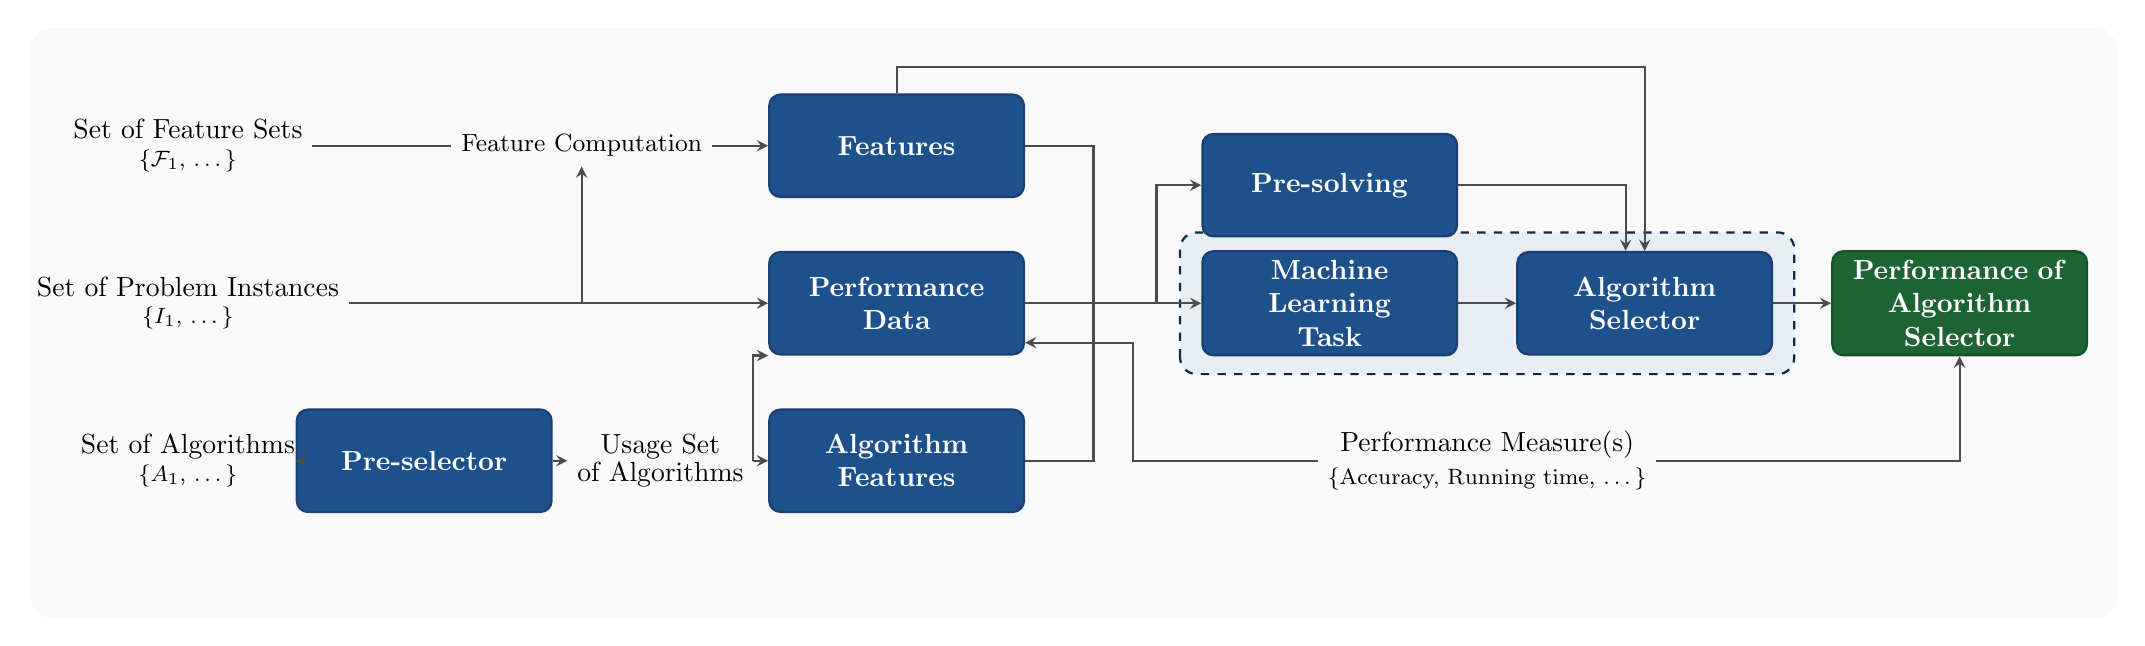
\begin{tikzpicture}[>=stealth, font=\normalsize]

        \fill[gray!5, rounded corners=8pt] (-0.5, 0.0) rectangle (26.0, 7.5);
        \definecolor{pipelineblue}{RGB}{30, 80, 140}
        \definecolor{evalgreen}{RGB}{30, 100, 50}
        \tikzset{
            data/.style={draw=pipelineblue!80!black, thick, fill=pipelineblue, text=white, rounded corners=4pt, text width=3.0cm, minimum height=1.3cm, align=center},
            process/.style={draw=pipelineblue!80!black, thick, fill=pipelineblue, text=white, rounded corners=4pt, text width=3.0cm, minimum height=1.3cm, align=center},
            eval/.style={draw=evalgreen!80!black, thick, fill=evalgreen, text=white, rounded corners=4pt, text width=3.0cm, minimum height=1.3cm, align=center},
            inputset/.style={align=center, font=\normalsize, text=black},
            metric/.style={align=center, font=\normalsize, text=black},
            arrow/.style={->, thick, draw=black!70},
            line/.style={thick, draw=black!70}
        }
        

        \fill[pipelineblue!10, rounded corners=6pt] (14.1, 3.1) rectangle (21.9, 4.9);
        \draw[dashed, pipelineblue!50!black, thick, rounded corners=6pt] (14.1, 3.1) rectangle (21.9, 4.9);
        \node[text=pipelineblue!80!black, font=\bfseries\scriptsize, anchor=south east] at (21.7, 3.25) {Core ML Pipeline};
        

        \node[inputset] (feat_sets) at (1.5, 6.0) {Set of Feature Sets\\[-0.5ex]\textnormal{\footnotesize \{$\mathcal{F}_1$, \dots\}}};
        \node[inputset] (instances) at (1.5, 4.0) {Set of Problem Instances\\[-0.5ex]\textnormal{\footnotesize \{$I_1$, \dots\}}};
        \node[inputset] (algos) at (1.5, 2.0) {Set of Algorithms\\[-0.5ex]\textnormal{\footnotesize \{$A_1$, \dots\}}};


        \node[process] (preselector) at (4.5, 2.0) {\textbf{Pre-selector}};
        \node[inputset] (usage_algos) at (7.5, 2.0) {Usage Set\\[-0.5ex]of Algorithms};


        \node[data] (features) at (10.5, 6.0) {\textbf{Features}};
        \node[data] (perf_data) at (10.5, 4.0) {\textbf{Performance}\\\textbf{Data}};
        \node[data] (algo_feats) at (10.5, 2.0) {\textbf{Algorithm}\\\textbf{Features}};


        \node[process] (ml_task) at (16.0, 4.0) {\textbf{Machine Learning}\\\textbf{Task}};
        \node[process] (presolving) at (16.0, 5.5) {\textbf{Pre-solving}};
        \node[process] (selector) at (20.0, 4.0) {\textbf{Algorithm}\\\textbf{Selector}};
        \node[eval] (perf_selector) at (24.0, 4.0) {\textbf{Performance of}\\\textbf{Algorithm Selector}};


        \node[metric] (perf_meas) at (18.0, 2.0) {Performance Measure(s)\\\textnormal{\footnotesize \{Accuracy, Running time, \dots\}}};



        \node[font=\small, text=black, fill=gray!5] (feat_comp) at (6.5, 6.0) {Feature Computation};
        \draw[line] (feat_sets.east) -- (feat_comp.west);
        \draw[arrow] (feat_comp.east) -- (features.west);
        \draw[arrow] (instances.east) -| (feat_comp.south);


        \draw[arrow] (algos) -- (preselector);
        \draw[arrow] (preselector) -- (usage_algos);
        

        \draw[arrow] (instances) -- (perf_data);
        \draw[arrow] (usage_algos.east) |- (perf_data.south west);
        \draw[arrow] (usage_algos.east) -- (algo_feats.west);


        \draw[line] (features.east) -| (13.0, 4.0);
        \draw[line] (algo_feats.east) -| (13.0, 4.0);
        \draw[line] (perf_data.east) -- (13.0, 4.0);
        \draw[arrow] (13.0, 4.0) -- (ml_task.west);


        \draw[arrow] (ml_task) -- (selector);
        \draw[arrow] (selector) -- (perf_selector);
        \draw[arrow] (features.north) |- (20.0, 7.0) -- (selector.north);
        \draw[arrow] (perf_data.east) -| (13.8, 5.5) -- (presolving.west);
        \draw[arrow] (presolving.east) -| (selector.110);


        \draw[arrow] (perf_meas.east) -| (perf_selector.south);
        \draw[arrow] (perf_meas.west) -| (13.5, 3.5) -- (perf_data.east |- 0, 3.5);

    \end{tikzpicture}
    }
    \caption[Algorithm selection pipeline]{Algorithm selection pipeline. A portfolio of complementary algorithms can first be chosen by pre-selection. In running-time scenarios, a short pre-solving schedule may solve easy instances before feature computation or before invoking the learned selector. Instance features, optional algorithm features, and performance data are then used to train and evaluate the algorithm selector.

    }
    \label{fig:ch02:asf_pipeline}
\end{figure}

Algorithm selection methods are integrated into \textit{algorithm selection pipelines}, which include several components:
\begin{itemize}
    \item \textbf{Pre-selection:} A subset of algorithms is selected from a larger candidate set. In most real-world scenarios, only a few algorithms contribute substantially to \gls{vbs} performance, yet having many candidates to choose from makes accurate selection harder and increases the risk of poor predictions. Pre-selection constructs a small, complementary portfolio. A prominent method for pre-selection is greedy selection based on marginal contributions~\citep{XuEtAl08}, where algorithms are iteratively added to the portfolio if they yield the largest improvement to the \gls{vbs} performance.


    \item \textbf{Pre-solving schedules:} For problems where the metric of interest is running time (e.g., $\mathcal{NP}$-complete problem solving), it is beneficial to first run a short schedule (\emph{i.e.}, a sequence of solvers, each executed with a specific cut-off time) of solvers to solve easy instances quickly, thereby avoiding unnecessary feature computation. Such methods use, for example, a greedy method to decide which algorithms to run~\citep{XuEtAl08}, or use an optimisation problem to find the optimal pre-solving schedule~\citep{HooEtAl12,KadEtAl11}.

    \item \textbf{Algorithm selection:} An algorithm (or a schedule of algorithms) is selected based on the computed features. This step typically involves a machine learning model. For example, there can be models that predict the performance for each instance~\citep{XuEtAl08,OztEtAl22}, models that predict the ranking of the algorithms~\citep{XuEtAl12,KerEtAl18}, formulating the problem as a recommendation task~\citep{MisSeb17} and other approaches.

\end{itemize}
Additionally, for algorithm selection, there is a need for two additional, problem specific components:
\begin{itemize}
    \item \textbf{Feature computation:} Representative features of the problem instance are computed and used as input to the learned selector. These features can be hand-crafted or learned from the data. The choice of features is crucial for the performance of the algorithm selector. For example, the SATzilla features are well-known to be a good representation of \gls{sat} instances~\citep{HutEtAl14,ShaHoo24}, while for machine learning datasets, there exists many features, such as the basic descriptors of~\citet{OztEtAl22} to more complicated features, that include advanced statistics, such as the ones implemented in PyMFE~\citep{AlcEtAl20}.

    \item \textbf{Evaluation metric:} This is an important component of algorithm selection, as it is used to evaluate the performance of the algorithm selector. While there exist broadly applicable metrics such as the performance of the \gls{vbs} and \gls{sbs}, their definition depends on the specific problem.


    Therefore, a problem-specific evaluation metric must be chosen that represents the performance of the algorithm. This can be, for example, accuracy, precision, recall, F1-score, AUC, running time and more, depending on the use-case.
\end{itemize}
An overview of the algorithm selection pipeline is presented in~\cref{fig:ch02:asf_pipeline}.




\subsection{Algorithm selection versus multi-class classification}
A common mistake among newcomers to algorithm selection is to treat it as a standard multi-class classification problem.
Although an algorithm selector predicts one algorithm from a finite set and 

can therefore be seen as performing a multi-class prediction task, training it as an ordinary multi-class classifier can yield sub-par performance, because it discards the performance of the algorithms relative to each other.

To see why, consider an instance where the performance gap between the best and the second-best algorithm is small.
In that case, selecting the second-best algorithm is a reasonable error.
A plain multi-class classifier, however, treats this outcome as equally wrong as choosing an algorithm that performs very poorly on the instance.
As we show in our ASlib experiments (\cref{sec:ch10:aslib_appendix}), multi-class classifiers can indeed perform far below the other methods in practice.


\section{Bayesian optimisation}


In this section, we define the \gls{hpo} problem and describe the working mechanisms of the \gls{bo} framework. 
We also cover related work on dynamic design choices related to the components of \gls{bo}, as well as using ensembles in \gls{bo}.

\subsection{Hyperparameter optimisation} Let $\mathcal{A}$ be a learning algorithm with $n$ hyperparameters, $\Lambda_{i}$ the domain of the $i$-th hyperparameter, and $\mathbf{\Lambda} = \Lambda_{1} \times \Lambda_{2} \times \dots \Lambda_{n}$ the overall hyperparameter configuration space. 
We denote a hyperparameter configuration by $\mathbf{\lambda} \in \mathbf{\Lambda}$, and the algorithm $\mathcal{A}$ with its hyperparameters instantiated to $\mathbf{\lambda}$ by $\mathcal{A}_{\mathbf{\lambda}}$.
Given a dataset $D$, the objective of \gls{hpo} is to find a hyperparameter configuration $\mathbf{\lambda}^{*}$ that minimises the loss $\mathcal{L}$ of a model fitted by algorithm $\mathcal{A}$ with hyperparameters $\mathbf{\lambda}$ on training data ${D}_{train}$, and evaluated on validation data ${D}_{validate}$, for a given loss function $\mathcal{L}$, \emph{i.e.},
\begin{equation}
\label{eq:ch02:def-hpo}
\mathbf{\lambda}^{*} \in \argmin_{\mathbf{\lambda} \in \mathbf{\Lambda}} 
\mathcal{L}(\mathcal{A}_{\mathbf{\lambda}}, {D}_{train}, {D}_{validate}) = \argmin_{\mathbf{\lambda} \in \mathbf{\Lambda}} c(\mathbf{\lambda})
\end{equation}
Here, $c(\mathbf{\lambda})$ is a shorthand for the loss function when $\mathcal{A}_{\mathbf{\lambda}}$ and $D$ are fixed.
Note that $c(\mathbf{\lambda})$ is a black-box function, without a closed-form expression nor analytic gradient information.

\subsection{Bayesian optimisation} 
\label{sec:ch02:bac_bo}
Bayesian optimisation (\gls{bo})~\citep{Mockus12,Garnett23,Frazier18,Kushner62,Kushner64} is a family of surrogate-based algorithms for efficient global optimisation of black-box problems.
\changed{Typically,} \gls{bo} consists of three main modules: an \emph{initial design}, \emph{i.e.}, in \gls{hpo}, a set of hyperparameter configuration candidates $\boldsymbol{\lambda} = (\lambda^{(1)},\ldots, \lambda^{(r)})$ and their evaluations 
$c(\boldsymbol{\lambda}) = (c(\lambda^{(1)}),\ldots, c(\lambda^{(r)}))$; a \emph{surrogate model} (fitted to the 

observations) that returns an approximation $\hat{c}(\mathbf{\lambda})$ of the unknown loss function $c(\mathbf{\lambda})$ while capturing the uncertainty in the prediction $\hat{\sigma}(\mathbf{\lambda})$ on unobserved points in the search space; and an \emph{acquisition function}, which is optimised to suggest solution candidates to be evaluated next, usually balancing exploration and exploitation of the search space.
\changed{\gls{bo} then evaluates the most promising candidates.} 

To approximate the expensive objective function, \gls{bo} typically employs a Gaussian process (GP) model as the surrogate. The GP model defines a distribution over functions on the configuration space $c(\lambda)\sim\mathcal{GP}_c(\mu(\lambda),k(\lambda,\lambda'))$, where 
$\mu(\cdot)$ 
is a mean function and 
$k(\cdot,\cdot)$
is a covariance function. If we consider an observation model 
$y_i = c(\lambda^{(i)}) + \varepsilon_i$
with normally distributed noise, 
$\varepsilon_i\sim\mathcal{N}(0,\sigma^2_\varepsilon)$, 
the predicted value by the GP model at one unknown configuration 
$\lambda$ will also follow a normal distribution with mean 
$\mu(\lambda)=K_{\lambda,\boldsymbol{\lambda}}(K_{\boldsymbol{\lambda},\boldsymbol{\lambda}}+\sigma^2_\varepsilon I)^{-1}\boldsymbol{y}$ and variance $\sigma^2(\lambda)=k(\lambda,\lambda)-K_{\lambda,\boldsymbol{\lambda}}(K_{\boldsymbol{\lambda},\boldsymbol{\lambda}}+\sigma^2_\varepsilon I)^{-1} K_{\boldsymbol{\lambda},\lambda}$, 
where $\boldsymbol{y}=(y_1,\ldots,y_r)$ is the vector of observations, $K_{\boldsymbol{\lambda},\boldsymbol{\lambda}}=[k(\lambda^{(i)},\lambda^{(j)})]_{\lambda^{(i)},\lambda^{(j)}\in\boldsymbol{\lambda}}$ is the covariance matrix, and $K_{\lambda,\boldsymbol{\lambda}}=[k(\lambda^{(i)},\lambda)]_{\lambda^{(i)}\in\boldsymbol{\lambda}}$ is the correlation vector for all samples.

GPs as a surrogate model inherently provide both the mean and the variance vector.

However, GPs are not the only surrogate model used in \gls{bo}. Another common choice for a surrogate model are tree-based models, 
such as random forests (RFs). 
Tree-based models traditionally predict only the mean of the given data (\emph{e.g.}, in a regression setting). 
In this case, the variance is defined based on the variance of the predictions of the leaves~\citep{HutEtAl11}. 
With $t(\lambda)$ being the prediction of a tree $t \in T$, we calculate the mean $\mu(\lambda)$ and variance $\sigma(\lambda)$ for a set of trees $T$ as follows:

\begin{equation}
    \mu(\lambda)=\frac{1}{|T|} \cdot \sum_{t\in T} t(\lambda) \; ,
\end{equation}
\begin{equation}
    \sigma(\lambda)=\frac{1}{|T|} \cdot \sum_{t\in T} (t(\lambda) - \mu(\lambda))^2 \; .
\end{equation}





Alternatively, uncertainty can be estimated via quantile regression~\citep{KoeBas78}, using two separate models to predict the upper and lower quantile of the output distribution, and deriving variance from the spread between these quantiles.
We adopt this approach to estimate uncertainty for another tree-based model, gradient boosting (GB); this is done similarly to the implementation in the \textsc{scikit-optimize} package.\footnote{\url{https://github.com/scikit-optimize/scikit-optimize}}



\Gls{bo} proceeds iteratively until a termination criterion is met. In each iteration, it optimises the acquisition function
by repeatedly querying the surrogate model to generate a pool of solution candidates. It then evaluates the most high-potential solutions (\emph{i.e.}, the solutions that maximise the acquisition function) from this pool,
refines the surrogate model based on the new observations, and updates the optimum if the new point improves upon the true function value of the best observation so far.

Among the many variants of \gls{bo} from the literature, in this work, we focus on the state-of-the-art method for \gls{hpo} to empirically evaluate our ensembling method: HEBO~\citep{CowEtAl22}.
HEBO (Heteroscedastic and Evolutionary Bayesian optimisation) is a \gls{bo}-based optimiser with several advancements 
\changed{
targeting each of the core \gls{bo} modules described above.
For the surrogate model, HEBO uses GP with two key transformations: a power transformation applied to the output observations $\boldsymbol{y}$ and a Kumaraswamy transformation applied to the input configurations $\boldsymbol{\lambda}$; 

jointly, these address heteroscedasticity in the noise $\epsilon$ and non-stationarity in the covariance matrix $K_{\boldsymbol{\lambda},\boldsymbol{\lambda}}$.
\citet{CowEtAl22} showed that these transformations enhance the ability of GPs to accurately approximate the mapping between configurations and corresponding performances, which is crucial for \gls{hpo}.


For the acquisition function, rather than optimising a single criterion, HEBO samples new candidate configurations by maximising MACE~\citep{LyuEtAl18}, a multi-objective acquisition function that simultaneously considers expected improvement (EI)~\citep{Mockus75}, probability of improvement (PI)~\citep{Kushner64}, and upper confidence bound (UCB)~\citep{ForEtAl08}, providing a more robust balance between exploration and exploitation of the search space than any single acquisition function alone.

Additional details on HEBO can be found in~\cref{sec:imp_det}.
}





\section{Chapter conclusion}

\paragraph{Connection to the thesis}~
The concepts introduced in this chapter provide the common language for the remainder of the dissertation.
Algorithm selection motivates the need for informative instance representations and robust performance models, while Bayesian optimisation motivates the study of surrogate models and the role of accuracy in decision making.
The next part therefore starts with the first dependency of any empirical performance model: the features and representations on which it is trained.
